\documentclass[11pt]{article}

\usepackage[margin=1in]{geometry}
\usepackage{amsmath, amssymb}
\usepackage{booktabs}
\usepackage{hyperref}
\usepackage{braket}
\usepackage{pgfplots}
\pgfplotsset{compat=1.18}

\title{CSE 4412: Introduction to Quantum Computing \\ Homework 1 --- Chapter 2 Exercises}
\author{}
\date{}

\begin{document}
\maketitle

\section*{Exercise 2.2}
\textbf{Statement.} Let $\ket{+} = \frac{1}{\sqrt{2}}(\ket{0} + \ket{1})$ and $\ket{-} = \frac{1}{\sqrt{2}}(\ket{0} - \ket{1})$. Compute $\braket{+|+}$, $\braket{+|-}$, and $\braket{-|-}$. What can you say about these two vectors? You may use the fact that $\ket{0}$ and $\ket{1}$ are orthonormal.

\textbf{Hint.} Expand each bracket using bilinearity of the inner product (distribute over the $\pm$ sums), then substitute $\braket{0|0}=\braket{1|1}=1$ and $\braket{0|1}=\braket{1|0}=0$. Once you have all three numbers, think about what ``normalized'' and ``orthogonal'' mean (Definitions in Section 2.1.2) and what it implies when two normalized, mutually orthogonal vectors span the whole space.

\textbf{Your answer:}

Expand each inner product using bilinearity, then substitute $\braket{0|0}=\braket{1|1}=1$ and $\braket{0|1}=\braket{1|0}=0$.
\[
\braket{+|+} = \frac{1}{\sqrt2}\cdot\frac{1}{\sqrt2}\big(\braket{0|0}+\braket{0|1}+\braket{1|0}+\braket{1|1}\big) = \frac12(1+0+0+1) = 1
\]
\[
\braket{+|-} = \frac{1}{\sqrt2}\cdot\frac{1}{\sqrt2}\big(\braket{0|0}-\braket{0|1}+\braket{1|0}-\braket{1|1}\big) = \frac12(1-0+0-1) = 0
\]
\[
\braket{-|-} = \frac{1}{\sqrt2}\cdot\frac{1}{\sqrt2}\big(\braket{0|0}-\braket{0|1}-\braket{1|0}+\braket{1|1}\big) = \frac12(1-0-0+1) = 1
\]
Since $\braket{+|+}=\braket{-|-}=1$, both $\ket{+}$ and $\ket{-}$ are normalized (unit vectors), and since $\braket{+|-}=0$, they are orthogonal to each other. Two normalized, mutually orthogonal vectors in a 2-dimensional space form an orthonormal basis, so $\{\ket{+},\ket{-}\}$ is an alternative orthonormal basis for the qubit state space (alongside $\{\ket{0},\ket{1}\}$).

\vspace{1cm}

\section*{Exercise 2.4}
\textbf{Statement.} Consider the following three questions:
\begin{enumerate}
    \item Consider the $\ket{+}$ state. What is the probability of observing $\ket{1}$ after a measurement?
    \item Consider $\ket{-} = \frac{1}{\sqrt{2}}(\ket{0} - \ket{1})$. What is the probability of observing $\ket{1}$ after measuring that state?
    \item Consider the state $\ket{1}$. What is the probability of observing $\ket{1}$ after measurement?
\end{enumerate}

\textbf{Hint.} For a state $\ket{\psi} = \alpha\ket{0} + \beta\ket{1}$, the rule from the chapter is $\Pr(\ket{1}) = |\beta|^2$, where $\beta$ is whatever is multiplying $\ket{1}$ once the state is written in the $\{\ket{0},\ket{1}\}$ basis. Identify $\beta$ in each of the three given states (watch the sign in $\ket{-}$ — remember you square the \emph{magnitude}).

\textbf{Your answer:}

For a state $\ket{\psi} = \alpha\ket{0} + \beta\ket{1}$, $\Pr(\ket{1}) = |\beta|^2$.
\begin{enumerate}
    \item $\ket{+} = \frac{1}{\sqrt2}\ket{0} + \frac{1}{\sqrt2}\ket{1}$, so $\beta = \frac{1}{\sqrt2}$ and
    \[
    \Pr(\ket{1}) = \left|\frac{1}{\sqrt2}\right|^2 = \frac12.
    \]
    \item $\ket{-} = \frac{1}{\sqrt2}\ket{0} - \frac{1}{\sqrt2}\ket{1}$, so $\beta = -\frac{1}{\sqrt2}$. Squaring the \emph{magnitude} discards the sign, so
    \[
    \Pr(\ket{1}) = \left|-\frac{1}{\sqrt2}\right|^2 = \frac12,
    \]
    the same probability as for $\ket{+}$, even though the two states are orthogonal (Exercise 2.2) -- the relative phase (sign) between $\alpha$ and $\beta$ does not affect the measurement probabilities in the computational basis.
    \item $\ket{1} = 0\cdot\ket{0} + 1\cdot\ket{1}$, so $\beta = 1$ and
    \[
    \Pr(\ket{1}) = |1|^2 = 1,
    \]
    i.e.\ measuring $\ket{1}$ always yields ``1'' with certainty, as expected since the state already is a computational basis state.
\end{enumerate}

\vspace{2cm}

\section*{Exercise 2.5}
\textbf{Statement.} Imagine you are given a qubit $\ket{\psi}$ but not told anything about it (i.e., you do not know its probability amplitudes). If you perform a measurement on the state and the outcome is ``0,'' what does this tell you about the state? Can you learn the original probability amplitudes? What if you are given as many copies of $\ket{\psi}$ as you want -- what can be said then?

\textbf{Hint.} Separate the question into two parts. (a) Single measurement: think about \emph{state collapse} — what do you know about the state right after the measurement, versus what you knew about it beforehand? Can one classical bit of outcome data pin down two continuous amplitudes $\alpha,\beta$? (b) Many copies: if you measured each copy and tallied the fraction of ``0'' vs. ``1'' outcomes, what would that fraction converge to as the number of copies grows (law of large numbers)? Does that let you recover $\alpha$ and $\beta$ exactly, or only something about their magnitudes? Also recall the no-cloning theorem (mentioned in the text, Section 2.5.4) — why can't you manufacture the extra copies yourself?

\textbf{Your answer:}

Write $\ket{\psi} = \alpha\ket{0} + \beta\ket{1}$ with unknown $\alpha,\beta \in \mathbb{C}$, $|\alpha|^2+|\beta|^2=1$.

\textbf{(a) Single measurement.} Before the measurement, the state carries two continuous, real degrees of freedom (e.g.\ $|\alpha|$ and the relative phase, since one global degree of freedom is fixed by normalization and another which the global phase is physically unobservable). A measurement in the computational basis produces only \emph{one classical bit} of outcome data (``0'' or ``1''), which cannot possibly encode two continuous parameters -- so a single outcome can never pin down $\alpha,\beta$ exactly. Concretely, observing ``0'' tells us only that $\alpha \ne 0$ (this outcome had nonzero probability $|\alpha|^2$), and by \emph{state collapse} the qubit is now \emph{exactly} $\ket{0}$, regardless of what $\alpha,\beta$ were beforehand. So the single measurement destroys the very information we wanted to learn: post-measurement the state is deterministically $\ket{0}$, and the original amplitudes are unrecoverable, whether they were, say, $(\alpha,\beta) = (1,0)$ or $(\alpha,\beta) = \left(\frac{1}{\sqrt2},\frac{1}{\sqrt2}\right)$ or anything else with $\alpha \ne 0$ -- all of these are consistent with having observed ``0.''

\textbf{(b) Many copies.} If instead we are handed $n$ independently prepared copies of the same unknown $\ket{\psi}$ and measure each one (in the computational basis), the fraction of ``0'' outcomes is a random variable whose expectation is $|\alpha|^2$. By the law of large numbers, as $n \to \infty$ this empirical fraction converges to $|\alpha|^2$ exactly (and the fraction of ``1'' outcomes converges to $|\beta|^2 = 1-|\alpha|^2$). So with enough copies we can estimate the \emph{magnitudes} $|\alpha|$ and $|\beta|$ to arbitrary precision. However, this still does not recover $\alpha$ and $\beta$ exactly: measuring only in the computational basis is blind to the \emph{relative phase} between $\alpha$ and $\beta$ (e.g.\ $\frac{1}{\sqrt2}(\ket{0}+\ket{1}) = \ket{+}$ and $\frac{1}{\sqrt2}(\ket{0}-\ket{1}) = \ket{-}$ give identical statistics in the $\{\ket{0},\ket{1}\}$ basis -- see Exercise 2.4 parts 1--2 -- yet are orthogonal states). To also determine the relative phase one needs additional copies measured in other bases (e.g.\ $\{\ket{+},\ket{-}\}$); doing so for a tomographically complete set of bases lets one reconstruct $\alpha,\beta$ up to the single remaining, physically unobservable global phase (i.e.\ $\ket{\psi}$ and $e^{i\theta}\ket{\psi}$ can never be distinguished by any measurement).

Finally, note why the problem insists the copies must be \emph{given} to us rather than something we produce ourselves: the \textbf{no-cloning theorem} (Section 2.5.4) says there is no physical process that takes one copy of an arbitrary, unknown state $\ket{\psi}$ and outputs two copies of it. So we cannot bypass part (a)'s limitation by measuring our single qubit, then cloning it before measuring again -- copies of an unknown state can only come from someone (or something) re-preparing the same state independently each time, not from duplicating the one qubit we hold.

\vspace{1cm}

\section*{Exercise 2.6}
\textbf{Statement.} Let $p \in [0,1]$ be a real number and consider the state
\[
\ket{\psi} = \sqrt{p}\,\ket{0} + \sqrt{1-p}\,\ket{1}.
\]
Answer the following: (1) probability of observing $\ket{0}$ for a given $p$; (2) probability of observing $\ket{-}$ for a given $p$; (3)--(4) graph both probability distributions as functions of $p$.

\textbf{Hint.} For (1), same rule as Exercise 2.4, just applied to $\ket{0}$ instead of $\ket{1}$. For (2), you can't just read off a coefficient because $\ket{-}$ isn't one of the two basis vectors $\ket{\psi}$ is written in terms of — instead use the inner-product rule $\Pr(\ket{-}) = |\braket{-|\psi}|^2$ from Section 2.3.1 (Equation 2.36), and expand $\braket{-|\psi}$ using linearity and the known values of $\braket{0|0},\braket{0|1},\braket{1|0},\braket{1|1}$. For (3)-(4), once you have closed-form expressions in terms of $p$, you can plot them with pgfplots (\texttt{\textbackslash usepackage\{pgfplots\}}) or by hand on $[0,1]$ — try a few sample points ($p=0,\tfrac12,1$) first to sanity-check the shape before you commit to plotting code.

\textbf{Your answer:}

\textbf{(1) Probability of observing $\ket{0}$.} Writing $\ket{\psi} = \alpha\ket{0}+\beta\ket{1}$ with $\alpha=\sqrt{p}$, the rule from Exercise 2.4 (applied to $\ket{0}$ instead of $\ket{1}$) gives
\[
\Pr(\ket{0}) = |\alpha|^2 = \left|\sqrt{p}\right|^2 = p.
\]
(Sanity check: $p=0 \Rightarrow \ket{\psi}=\ket{1} \Rightarrow \Pr(\ket 0)=0$; $p=1 \Rightarrow \ket{\psi}=\ket 0 \Rightarrow \Pr(\ket 0)=1$. Both match $\Pr(\ket0)=p$.)

\textbf{(2) Probability of observing $\ket{-}$.} Since $\ket{-}$ is not one of the two basis vectors $\ket{\psi}$ is expanded in, use $\Pr(\ket{-}) = |\braket{-|\psi}|^2$. Expand $\bra{-} = \frac{1}{\sqrt2}(\bra0-\bra1)$ against $\ket\psi = \sqrt p\,\ket0+\sqrt{1-p}\,\ket1$:
\[
\braket{-|\psi} = \frac{1}{\sqrt2}\Big(\sqrt p\,\braket{0|0} + \sqrt{1-p}\,\braket{0|1} - \sqrt p\,\braket{1|0} - \sqrt{1-p}\,\braket{1|1}\Big)
= \frac{1}{\sqrt2}\big(\sqrt p - \sqrt{1-p}\big).
\]
Squaring the magnitude,
\[
\Pr(\ket{-}) = \big|\braket{-|\psi}\big|^2 = \frac12\big(\sqrt p-\sqrt{1-p}\big)^2
= \frac12\Big(p + (1-p) - 2\sqrt{p(1-p)}\Big)
= \frac12 - \sqrt{p(1-p)}.
\]
(Sanity check: $p=\tfrac12 \Rightarrow \ket\psi=\ket+$, and $\Pr(\ket-) = \tfrac12-\tfrac12=0$, correct since $\ket+\perp\ket-$. At $p=0$ or $p=1$, $\ket\psi\in\{\ket0,\ket1\}$ and $\Pr(\ket-)=\tfrac12-0=\tfrac12$, correct since $\ket0,\ket1$ each have overlap $\tfrac{1}{\sqrt2}$ with $\ket-$.)

\textbf{(3)--(4) Plots.} Both are functions of $p\in[0,1]$: $\Pr(\ket0)=p$ is a straight line from $(0,0)$ to $(1,1)$; $\Pr(\ket-)=\tfrac12-\sqrt{p(1-p)}$ is symmetric about $p=\tfrac12$, equal to $0$ at $p=\tfrac12$ (its minimum) and rising to $\tfrac12$ at both endpoints $p=0,1$ (its maximum) -- an upside-down ``dome'' turned into a ``valley''.
\begin{center}
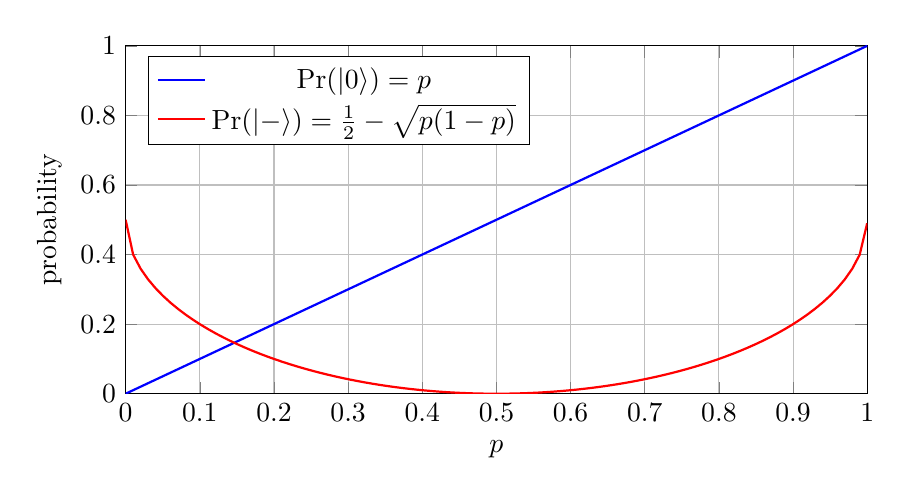
\begin{tikzpicture}
\begin{axis}[
    width=11cm, height=6cm,
    xlabel={$p$}, ylabel={probability},
    xmin=0, xmax=1, ymin=0, ymax=1,
    legend pos=north west, grid=major,
]
\addplot[domain=0:1, samples=100, thick, blue] {x};
\addlegendentry{$\Pr(\ket{0}) = p$}
\addplot[domain=0:1, samples=100, thick, red] {0.5 - sqrt(x*(1-x))};
\addlegendentry{$\Pr(\ket{-}) = \tfrac12 - \sqrt{p(1-p)}$}
\end{axis}
\end{tikzpicture}
\end{center}

\vspace{1cm}

\section*{Exercise 2.8}
\textbf{Statement.} Let $\ket{\psi}$ be some $d$-dimensional state and let $\mathcal{B} = \{\ket{b_0}, \dots, \ket{b_{d-1}}\}$ be any orthonormal basis. Show that $\ket{\psi}$ may be written as
\[
\ket{\psi} = \sum_{j=0}^{d-1} \braket{b_j|\psi}\,\ket{b_j}.
\]

\textbf{Hint.} This is essentially asking you to re-derive the \emph{completeness relation} argument from Section 2.1.3 (Equation 2.22-2.23). Start from the fact that $\sum_j \ket{b_j}\bra{b_j} = I$ for any orthonormal basis, apply both sides to $\ket{\psi}$, and note that $\ket{b_j}\bra{b_j}\ket{\psi}$ can be regrouped as a scalar $\braket{b_j|\psi}$ times the vector $\ket{b_j}$.

\textbf{Your answer:}

Since $\mathcal{B} = \{\ket{b_0},\dots,\ket{b_{d-1}}\}$ is a basis for the $d$-dimensional space, every vector in that space -- including $\ket\psi$ -- can be written as \emph{some} linear combination of the $\ket{b_j}$:
\[
\ket\psi = \sum_{j=0}^{d-1} c_j \ket{b_j}, \qquad \text{for some (as yet unknown) scalars } c_j \in \mathbb{C}.
\]
To identify the coefficients $c_j$, take the inner product of both sides with an arbitrary basis bra $\bra{b_k}$:
\[
\braket{b_k|\psi} = \sum_{j=0}^{d-1} c_j \braket{b_k|b_j}.
\]
Because $\mathcal B$ is \emph{orthonormal}, $\braket{b_k|b_j} = \delta_{kj}$ (i.e.\ $1$ if $k=j$, $0$ otherwise), so every term in the sum vanishes except $j=k$:
\[
\braket{b_k|\psi} = c_k.
\]
This holds for every $k=0,\dots,d-1$, so the unknown coefficients are exactly $c_j = \braket{b_j|\psi}$. Substituting back into the original expansion gives
\[
\ket\psi = \sum_{j=0}^{d-1} \braket{b_j|\psi}\,\ket{b_j},
\]
as required. Equivalently, this is the statement that $\sum_j \ket{b_j}\bra{b_j} = I$ (the \emph{completeness relation}): applying this operator identity to $\ket\psi$ gives $\ket\psi = I\ket\psi = \sum_j \ket{b_j}\bra{b_j}\ket\psi$, and regrouping each term $\ket{b_j}\big(\bra{b_j}\ket\psi\big)$ as the scalar $\braket{b_j|\psi}$ times the vector $\ket{b_j}$ recovers the same formula. This is exactly why $\braket{b_j|\psi}$ is called the ``component of $\ket\psi$ along $\ket{b_j}$'' -- it plays the same role as a dot product picking out coordinates in ordinary vector geometry, just generalized to any orthonormal basis of the state space (not only $\{\ket0,\ket1\}$).

\end{document}
